%----------------------------------------------------------
\def\notedate{2022.09.29}
\def\currentauthor{Василян А.Р. (РК6-73Б)}
%----------------------------------------------------------
\notestatement{rndhpcgui}{Программный инструментарий для создания подсистем ввода данных при разработке систем инженерного анализа}

%---------------------------------------------------------

В результате анализа статьи \cite{Sokolov2017} были изучены основные определения, программный инструментарий. Автоматическое построение GUI -- построение графических форм ввода исходных данных для прикладной программы без участия человека с использованием программы-генератора GUI и файла исходных данных в специальном формате; Метаданные -- список входных параметров и их текущие значения в рамках выполнения прикладной программой вычислительной задачи.

На рисунке~\ref{rndhpcgui.2022.09.29.diagram} представлена диаграмма потока данных при построении и эксплуатации GUI на основе созданного программного инструментария и формата aINI. Описание некоторых процедур в схеме:
\begin{enumerate} [start=0]
	\item процедура создания и редактирования списка входных данных осуществляется вручную с использованием доступных текстовых редакторов в формате aINI.
	\item чтение aINI-файла осуществляется aINI-парсером, обеспечивающим синтаксический разбор конструкций aINI-файла, включая типы каждого параметра, и формирование aINI-объекта.
	\item построение GUI осуществляется с помощью платформозависимого GUI-генератора, на вход которого подается aINI-объект во время выполнения прикладной программы, использующей соответствующий aINI-файл в качестве входных данных.
	\item автоматическое обновление aINI-файла согласно внесенным пользователем изменениям в значения входных параметров в экранной форме. 
	\item процедура ввода данных включает изменение текущих значений входных параметров и осуществляется в сформированной экранной форме. Количество и типы входных параметров при этом не изменяются.
	\item создание объекта класса AnyMap, содержащего все входные параметры и их текущие значения (метаданные), осуществляется для возможности дальнейшей передачи на вход функциям обработки данных или для возможности передачи по сети на удаленный высокопроизводительный узел с целью проведения расчета на нем.
	\item обновление объекта исходных данных класса AnyMap осуществляется после изменения значений в экранных формах.
	\item непосредственная обработка объекта исходных данных класса AnyMap.
\end{enumerate}

\begin{figure}[!ht]
  \centering
  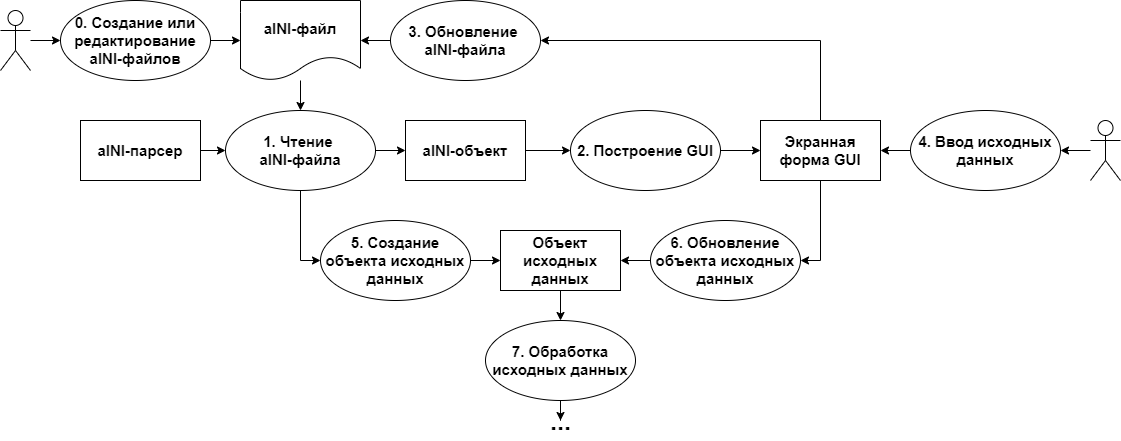
\includegraphics[scale=0.35]{ResearchNotes/rndhpc_int_gui_2022_09_29/rndhpcgui.2022.09.29.diagram.png}
  \caption{Диаграмма потока данных при построении и эксплуатации GUI на основе созданного программного инструментария и формата aINI}
  \label{rndhpcgui.2022.09.29.diagram}
\end{figure}

После изучения статьи в качестве языка определения входных данных был выбран aINI, так как подготовка входных данных доступна для неподготовленного специалиста, не владеющего навыками программирования, в том числе для специалистов, представляющих заказчика разрабатываемой прикладной программы. Формат основан на известном языке INI.
%----------------------------------------------------------
% Атрибуты задачи
\noteattributes{}
%----------------------------------------------------------

